\section{Feature Extraction}
Features are inherent properties of data, independent of coordinate frames.

Dimensions of a feature:
\begin{description}
\item 0: \emph{Point Feature} (often defined by $n$ equations of $n$ coordinates)
\item 1: \emph{Line-like feature} (n-1 equations)
\item 2: \emph{Surface-like feature}
\item n: \emph{region-type feature} (typically defined by a single inequality).
\end{description}

\subsection{Region-Type Features}
A feature is often indicated by high or low values of a \emph{derived field}. 

Example: \emph{vortical regions} in a flow field have been defined by:
\begin{itemize}
\item Large magnitude of \emph{vorticity}
    \begin{align*}
        \omega(x) = \Delta \times v(x).
    \end{align*}
\item High absolute \emph{helicity} 
    \begin{align*}
         \omega(x) \cdot v(x),
    \end{align*}
     or \emph{normalised helicity}:
     \begin{align*}
         { \omega(x)\over \norm{\omega(x)}} \cdot {v(x)\over \norm{v(x)}}.
     \end{align*}
\item Positive \emph{pressure Laplacian} 
    \begin{align*}
        \Delta \cdot \Delta p(x).
    \end{align*}
\item Positive \emph{second invariante} $Q$ of the velocity gradient $\Delta v(x)$.
\item Two negative \emph{eigenvalues} of
    \begin{align*}
        {\Delta v(x)^2 + (\Delta v(x)^T )^2 \over 2}.
    \end{align*}
\end{itemize}

\begin{figure}[H]
\centering
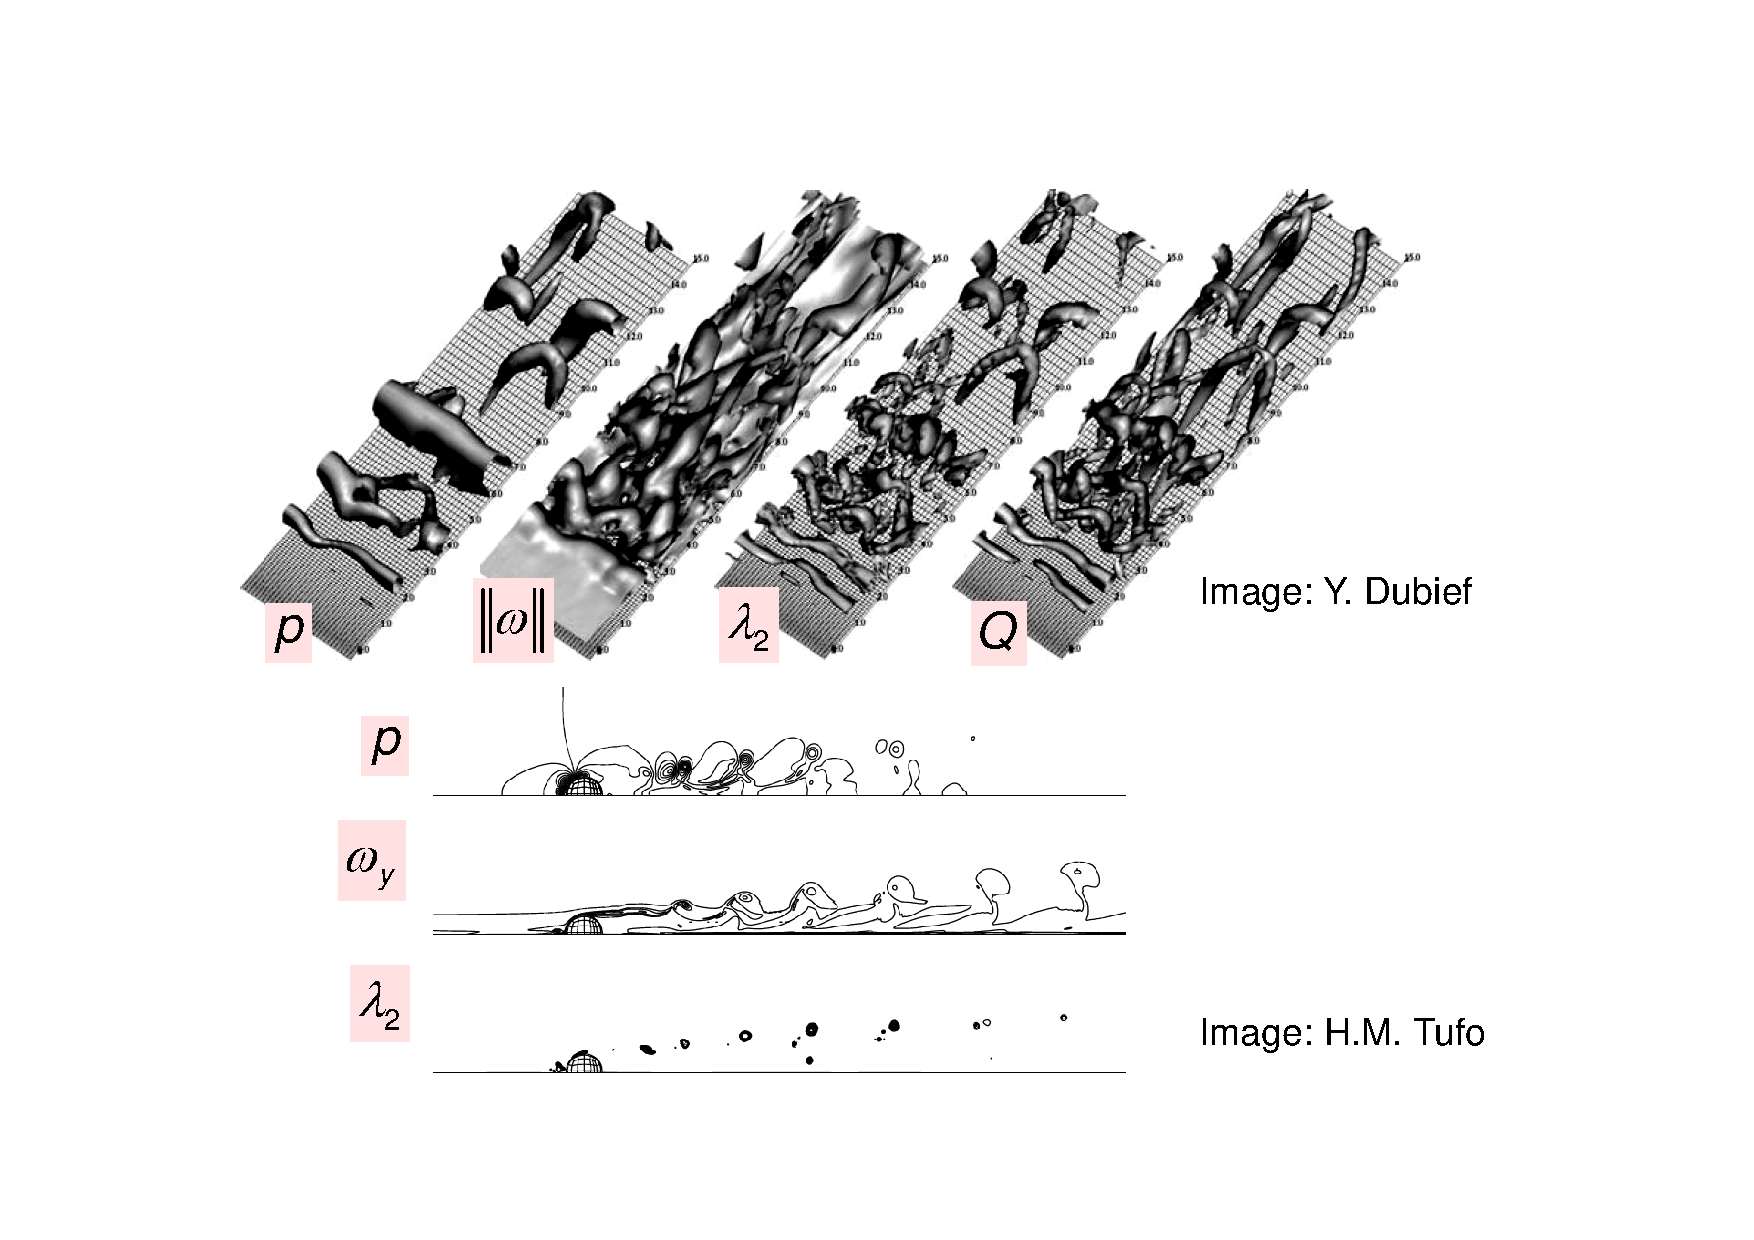
\includegraphics[width=0.8\textwidth]{img/07_region_features}
\end{figure}

\subsection{Point Features in Scalar Fields}
Point features in scalar fields:
\begin{itemize}
    \item Local minima/maxima
    \item Saddle points
\end{itemize}
occur at places where the height field is horizontal ($\Delta s(x)=0$)
\begin{figure}[H]
\centering
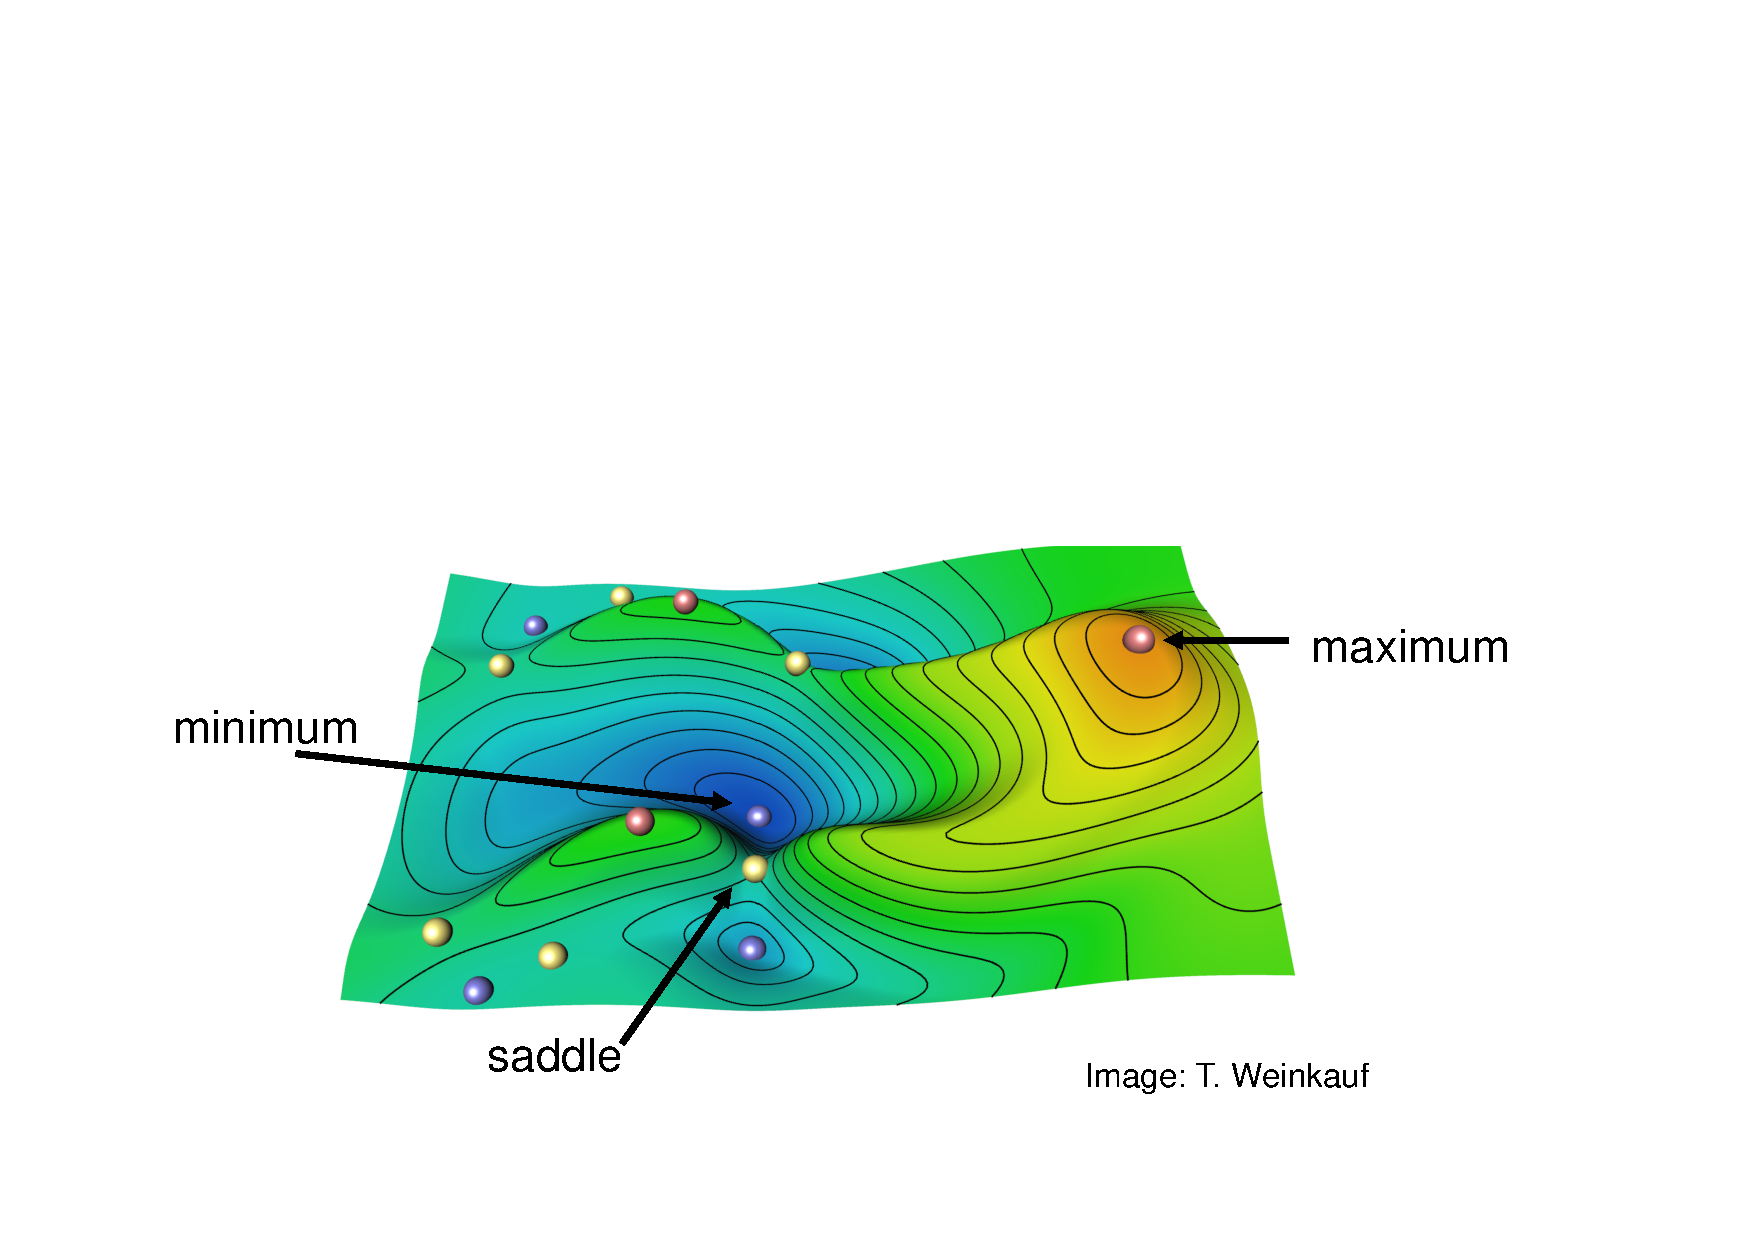
\includegraphics[width=0.6\textwidth]{img/07_scalar_features}
\end{figure}

These point features are the places where the isoline or isosurface changes its topology when the level is varied. 

The \emph{contour tree} or \emph{Reeb graph} describes the \em split, join, creation \em and \em deletion events\em.

\begin{figure}[H]
    \centering
    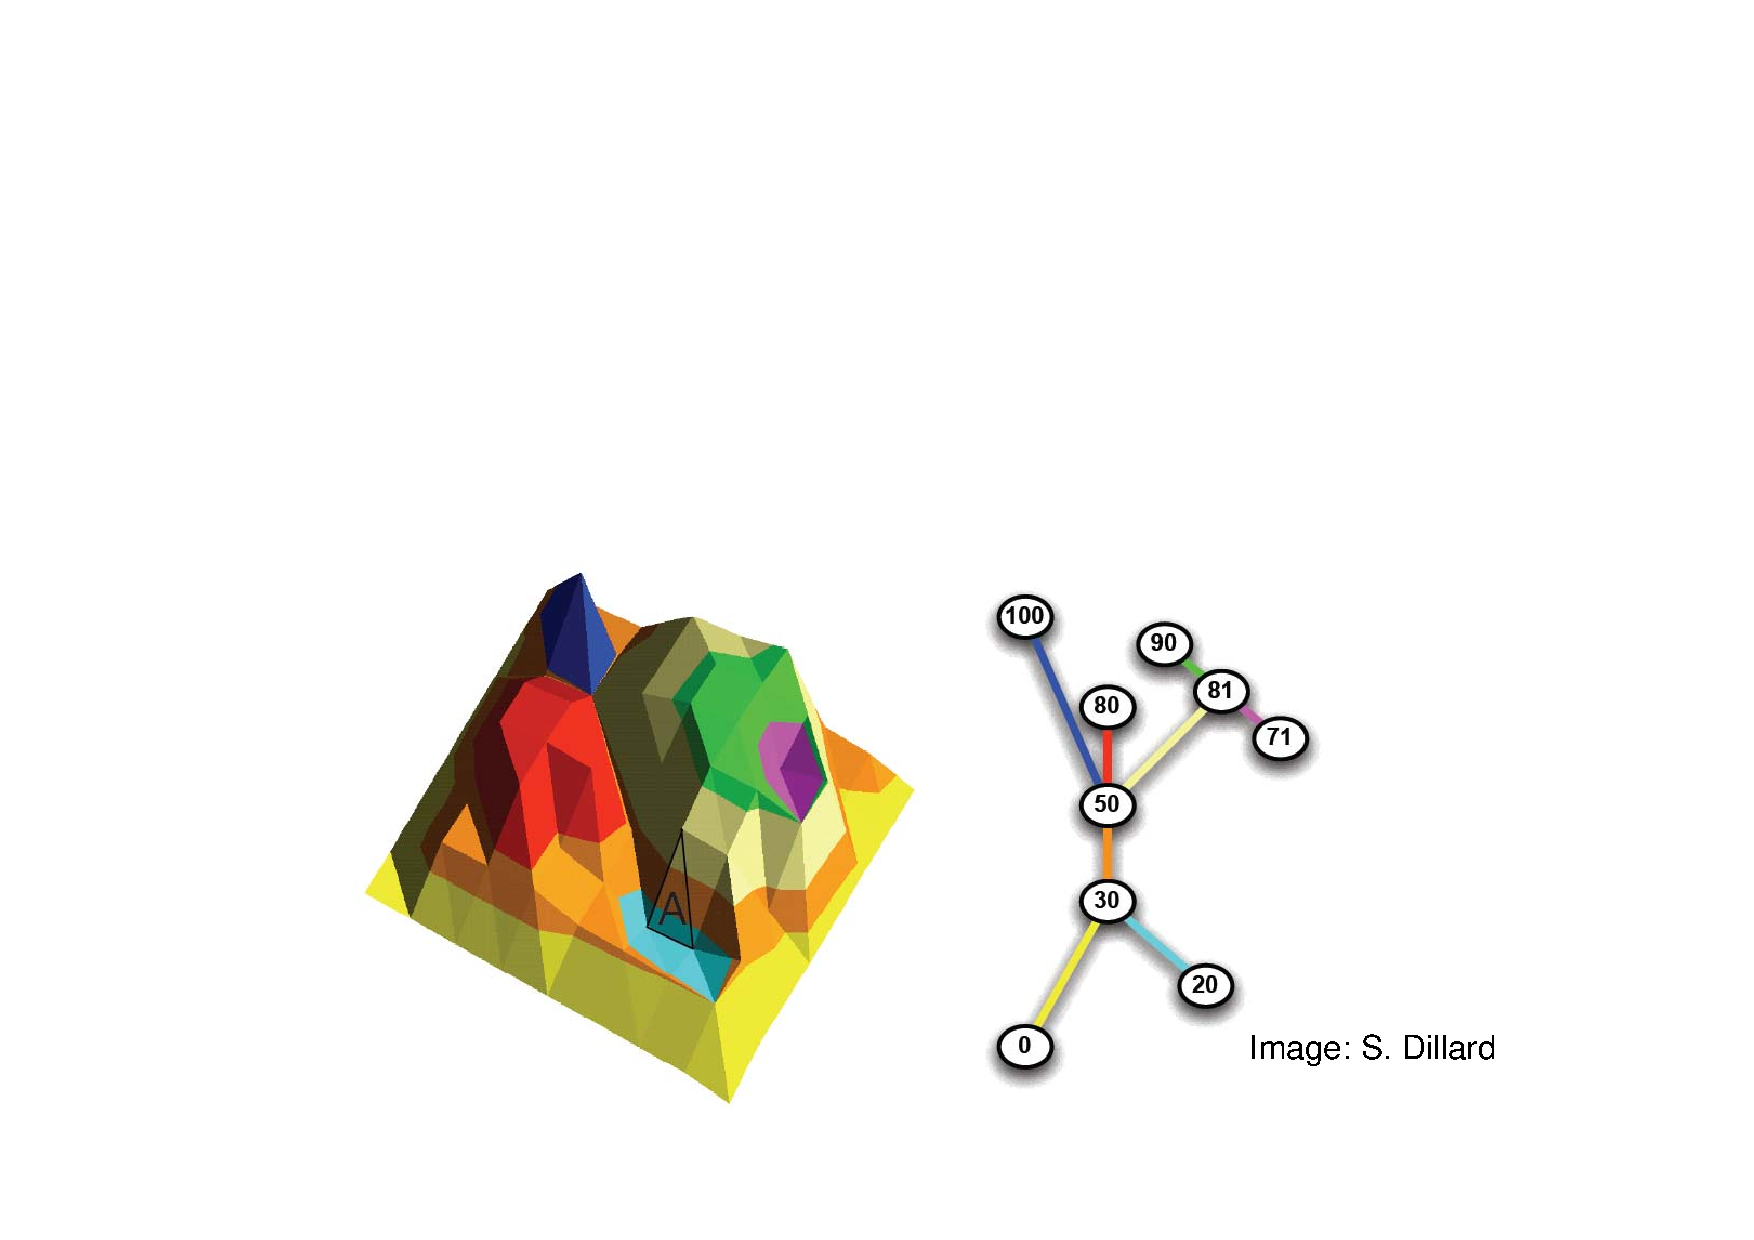
\includegraphics[width=0.7\textwidth]{img/07_contour_tree}
    \caption{Contour tree}
\end{figure}

\subsection{Line-Like Features in Scalar Fields}
\emph{Watersheds} describe ridges/valleys of a height field $s(x)$:
Integrate the \emph{gradient field} $\Delta s(x)$ (backward/forward) starting from \emph{saddle points}.

The watersheds provide a \emph{segmentation} of the domain into so-called \emph{Morse-Smale cells}.
\begin{figure}[H]
\centering
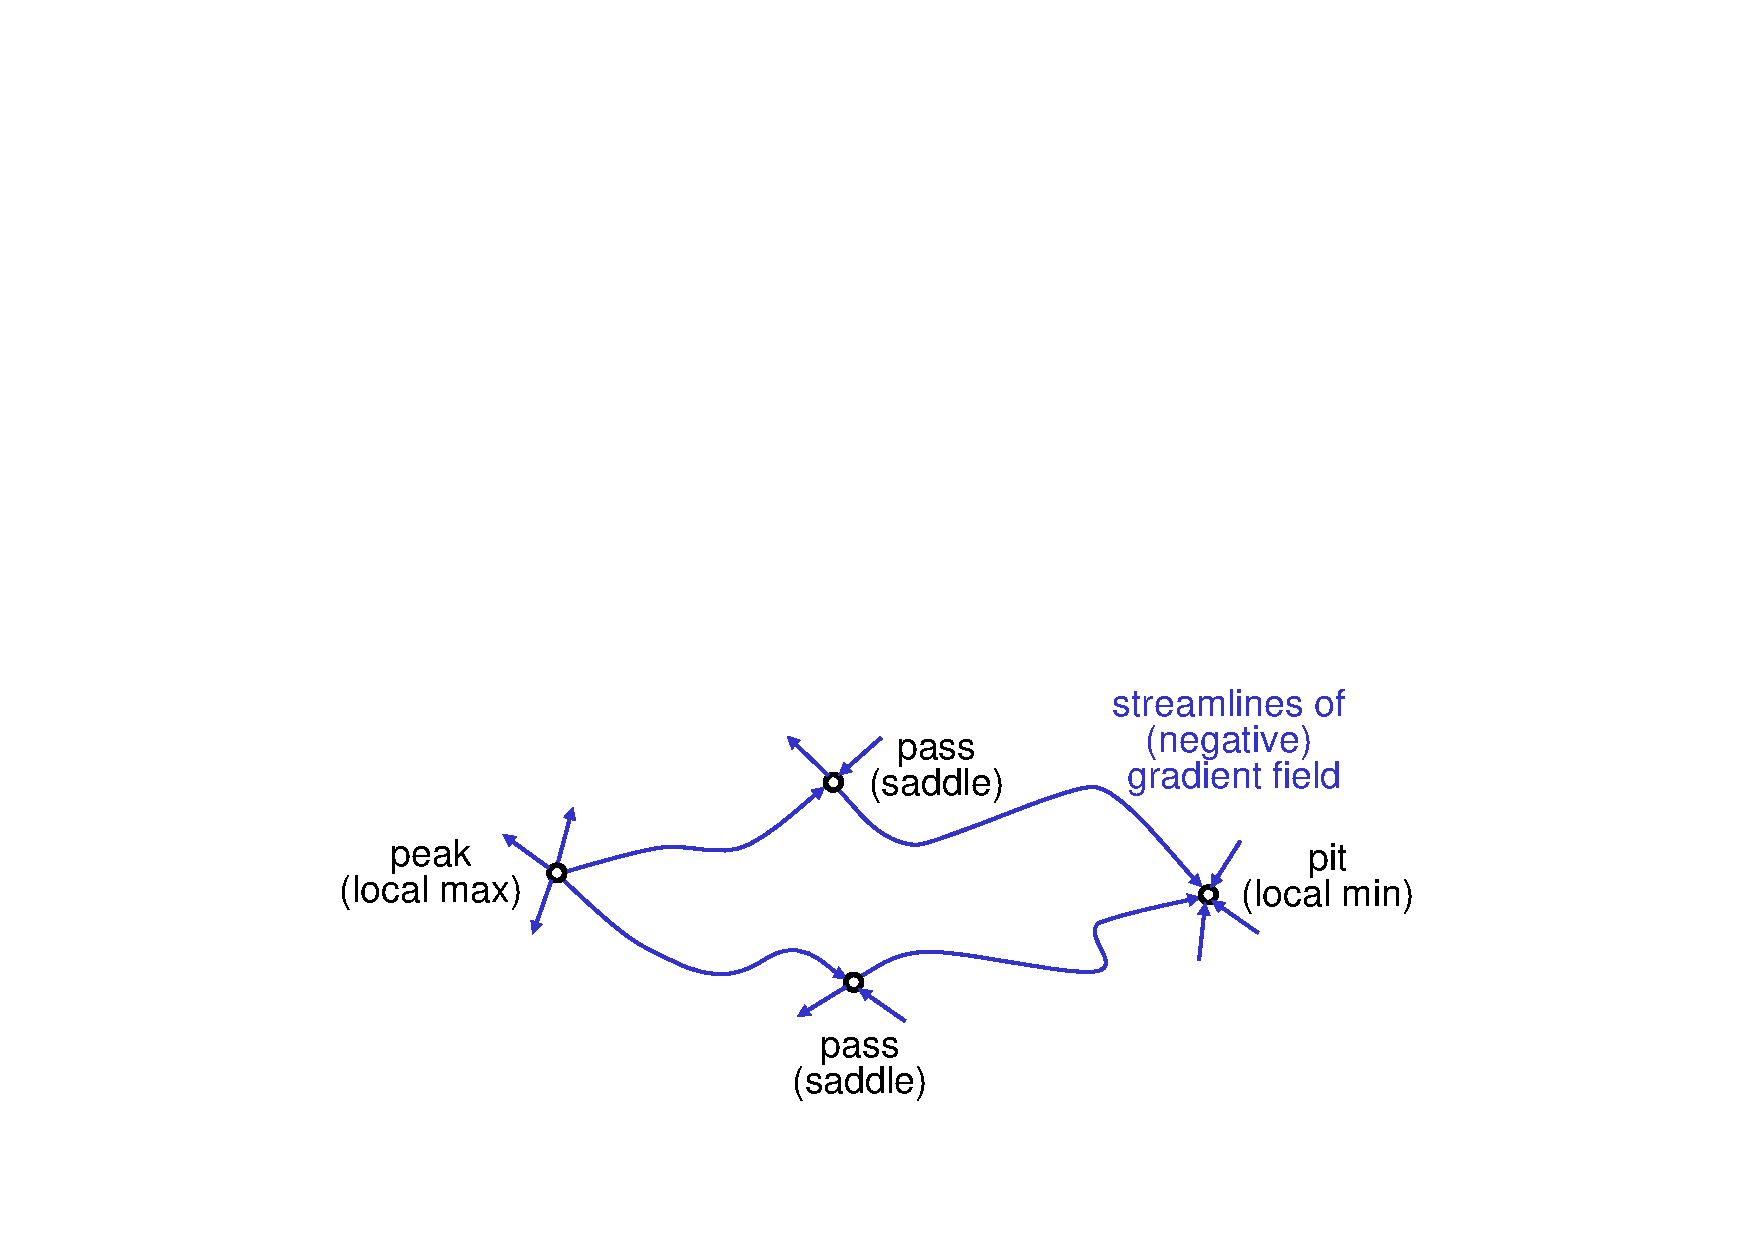
\includegraphics[width=0.6\textwidth]{img/07_watersheds}
\end{figure}

Watersheds require integration and are therefore not locally detectable. 


Often used concepts:
\begin{itemize}
    \item Section-based ridges
    \item Curvature extrema on height contours.
\end{itemize}

\paragraph{Height Ridges}
"Most natural extensions of local maxima to 1D features". 

A formal definition of height ridges was given only in the 1990s (Eberly, Lindeberg) based on Haralicks's definition (1983).

At a given point $x_0$ the scalar field has the Taylor approximation:
\begin{align*}
    s(x_0+x) = s(x_0)+\Delta s\cdot x + x^THx + \mathcal O(|x|^3),
\end{align*}
where $H$ is the \emph{Hessian} matrix of second derivatives
\begin{align*}
 H = \left( {\delta^2 s(x)\over \delta x_i \delta x_j}\right).
\end{align*}
With $H$ having real eigenvalues and orthogonal eigenvectors. By taking the eigenvectors as the coordinate frame $H$ becomes the diagonal matrix:
\begin{align*}
    H = 
        \begin{pmatrix}
             \lambda_1 & & 0\\
             & \ddots\\
             0 & & \lambda_n
        \end{pmatrix}.
\end{align*}
 A point $x\in \R^n$ is a \emph{local maximum} of $s(x)$ if \emph{for all n} axes if:
\begin{itemize}
 \item The first derivatives are zero:
     \begin{align*}
         s_{x_1} = ... = s_{x_n} = 0
     \end{align*}
 \item The second derivatives are negative:
     \begin{align*}
         s_{x_1 x_1}, ..., s_{x_n x_n} < 0.
     \end{align*}
\end{itemize}

In the appropriate coordinate frame this generalises to:

A point $x\in \R^n$ is on a $d$-dimensional \emph{height ridge} of $s(x)$ if \emph{for the first $n-d$} axes:
\begin{itemize}
 \item The first derivatives are zero:
     \begin{align*}
         s_{x_1} = ... = s_{x_n} = 0
     \end{align*}
 \item The second derivatives are negative:
     \begin{align*}
         s_{x_1 x_1}, ..., s_{x_n x_n} < 0.
     \end{align*}
\end{itemize}

"Appropriate coordinate frame" means that axes are:
\begin{itemize}
 \item Aligned with eigenvectors of $H$,
 \item Ordered by absolute eigenvalues
     \begin{align*}
         |\lambda_1| \geq \ldots \geq |\lambda_n|      \end{align*}
         (Lindeberg's version), or

     Ordered  by signed eigenvalues: 
     \begin{align*}
         \lambda_1 \leq \ldots \leq \lambda_n
     \end{align*}
\end{itemize}


\begin{figure}[H]
    \centering
    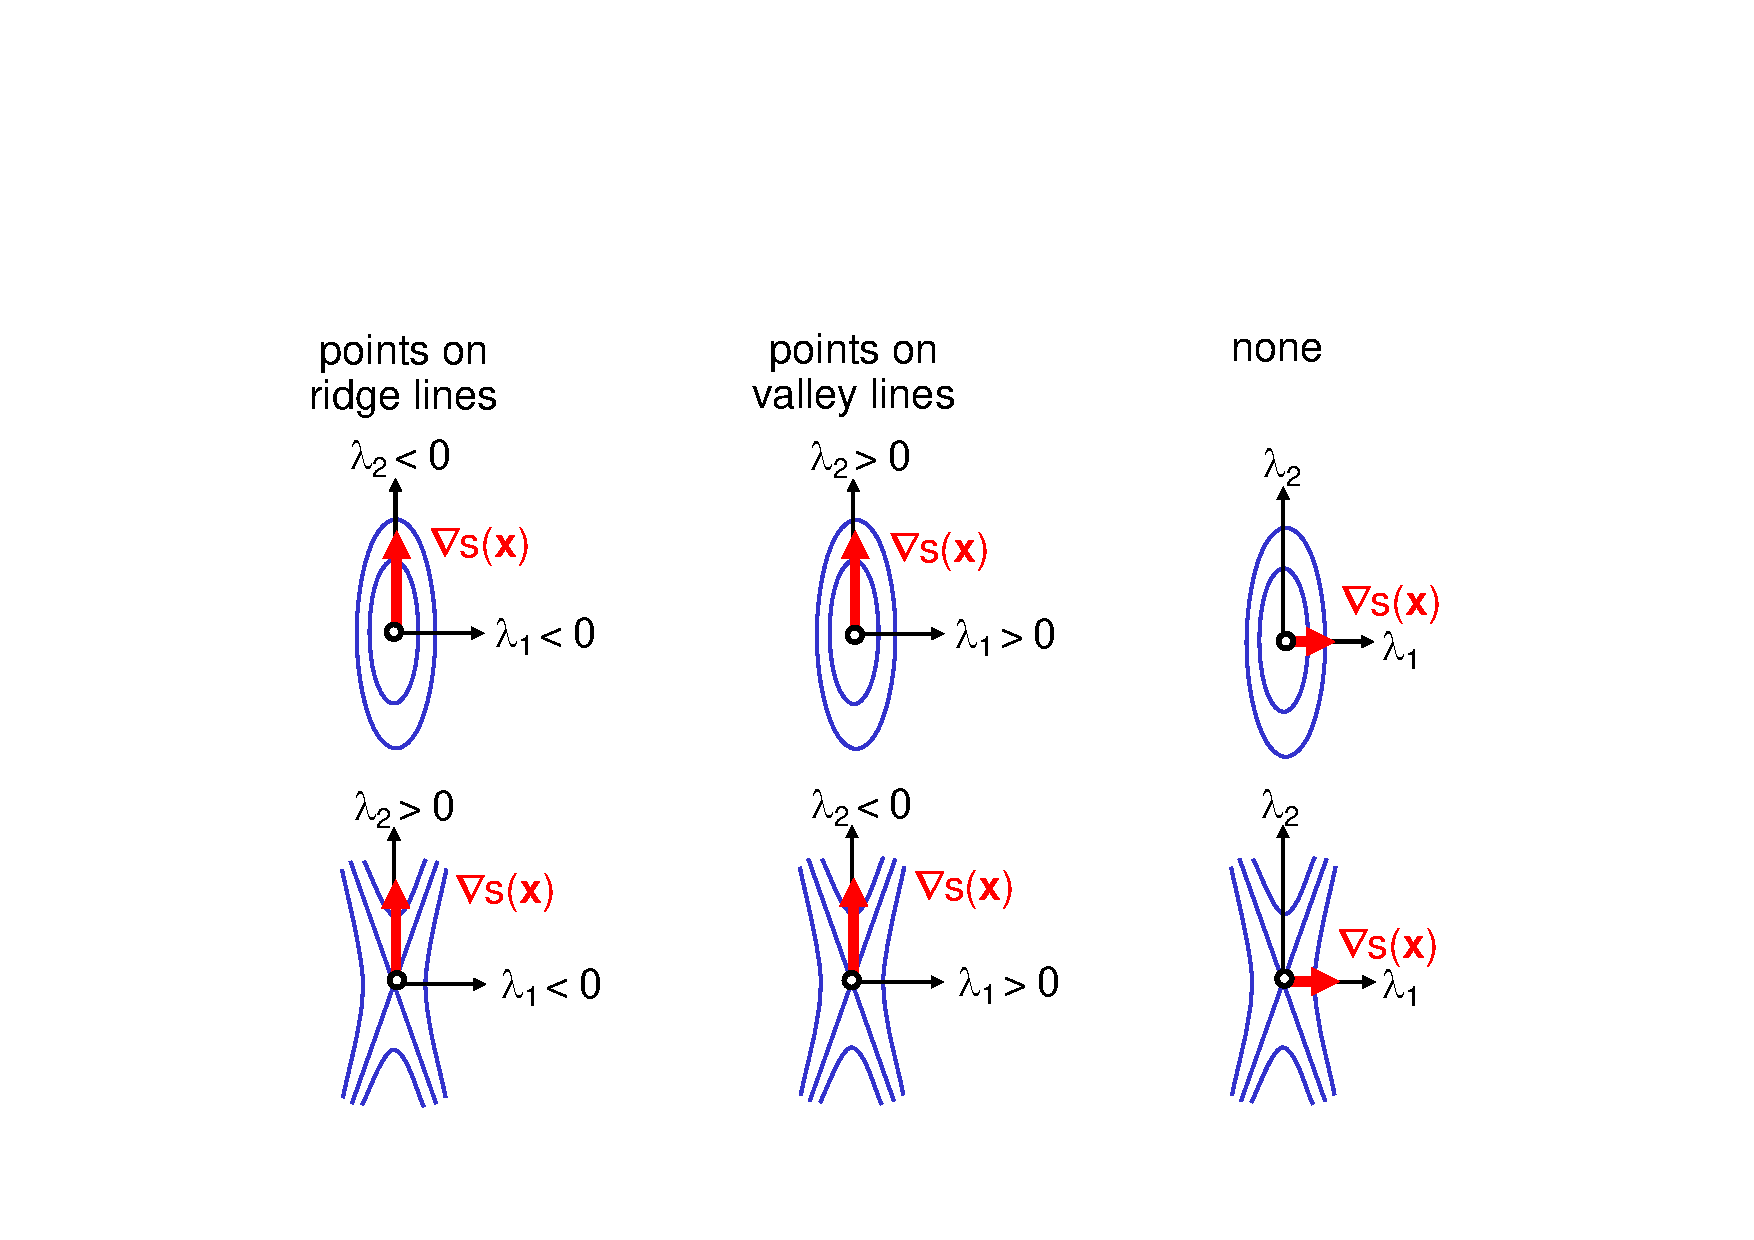
\includegraphics[width=0.7\textwidth]{img/07_lindeberg_cases}
\end{figure}

\subsubsection{Circular Gutter}
Example where slope lines and height ridge don't match. A "counter-example" for height ridges.
\begin{figure}[H]
    \centering
    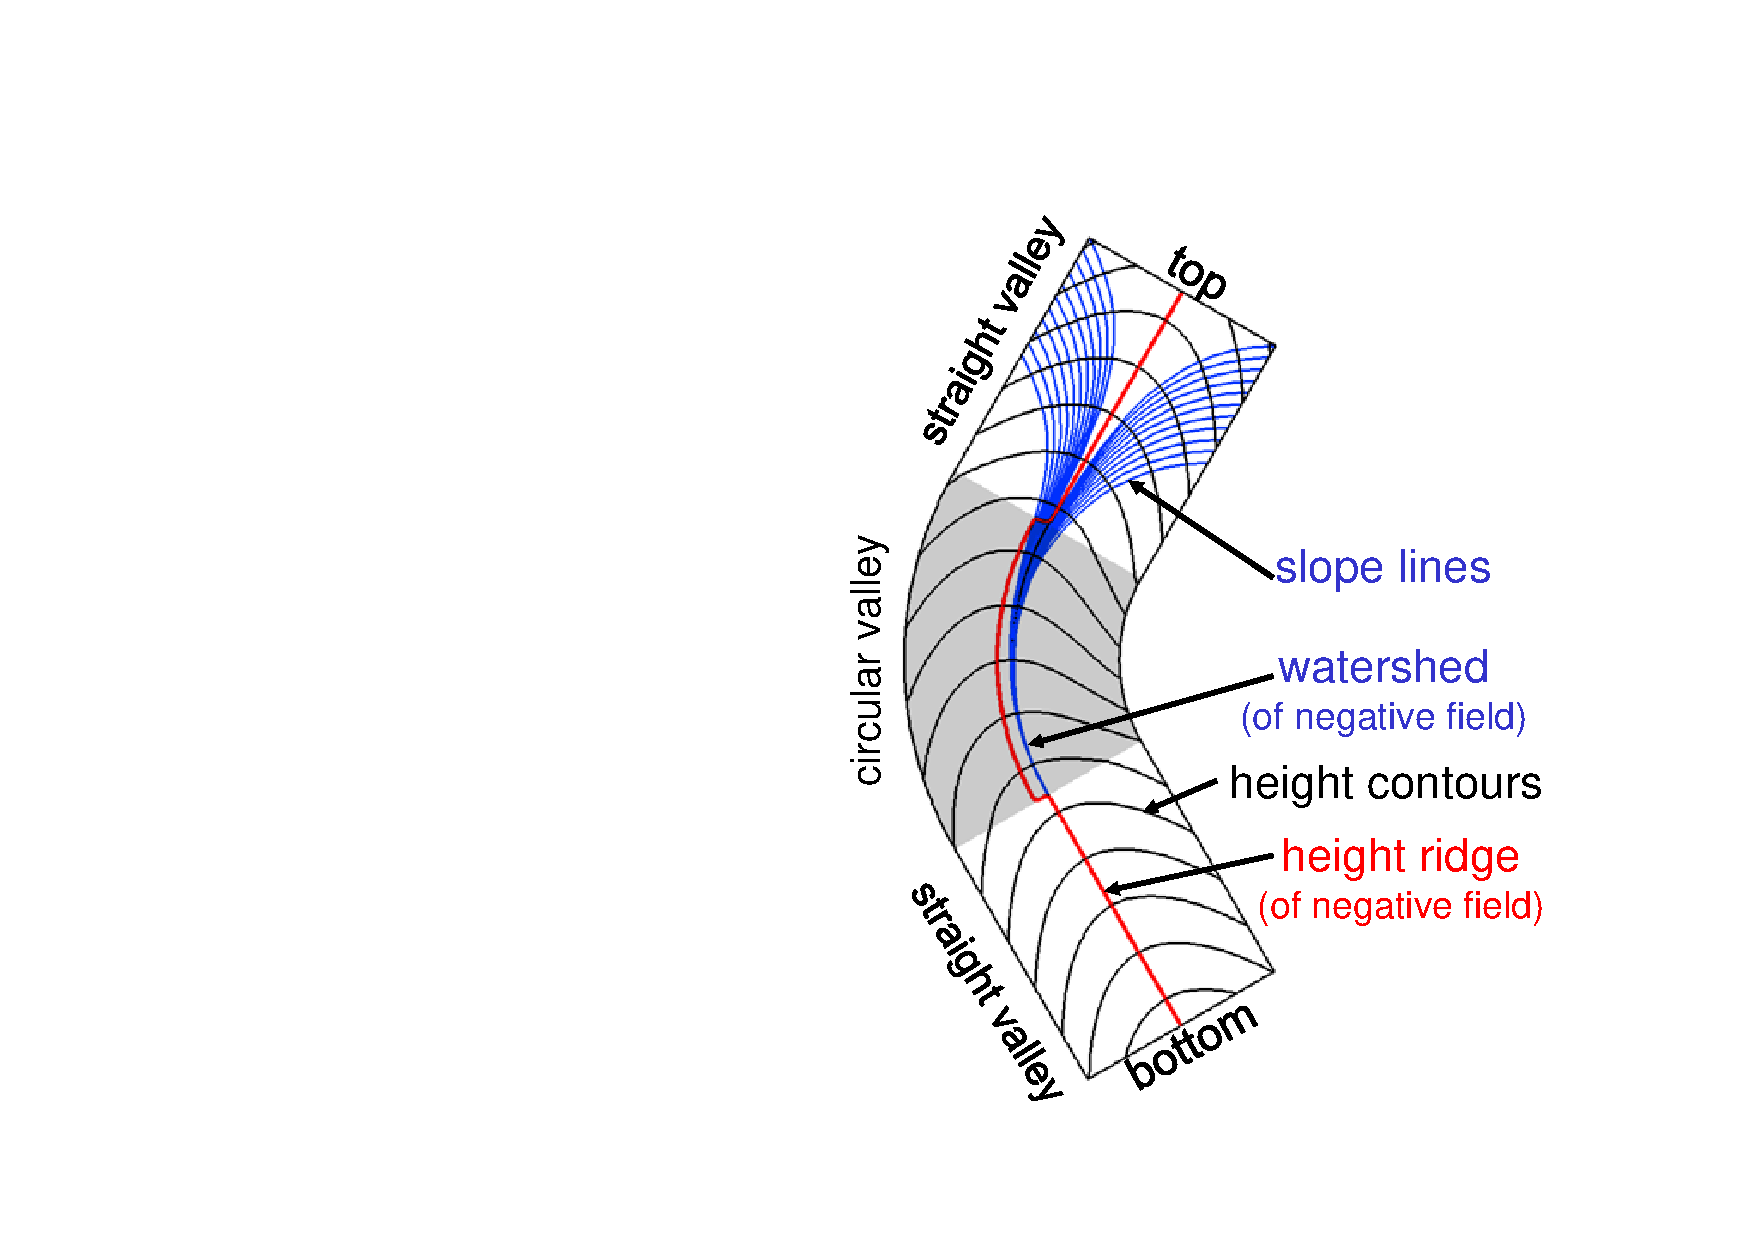
\includegraphics[width=0.4\textwidth]{img/07_gutter_example}
\end{figure}

\subsubsection{Blended Height Fields}
By replacing the circular part of the circular gutter by a blend of the two height fields we observe that the watershed deviates (in the lowerpart) from the obvious symmetric valley line. A "counter-example" for watersheds.
\begin{figure}[H]
    \centering
    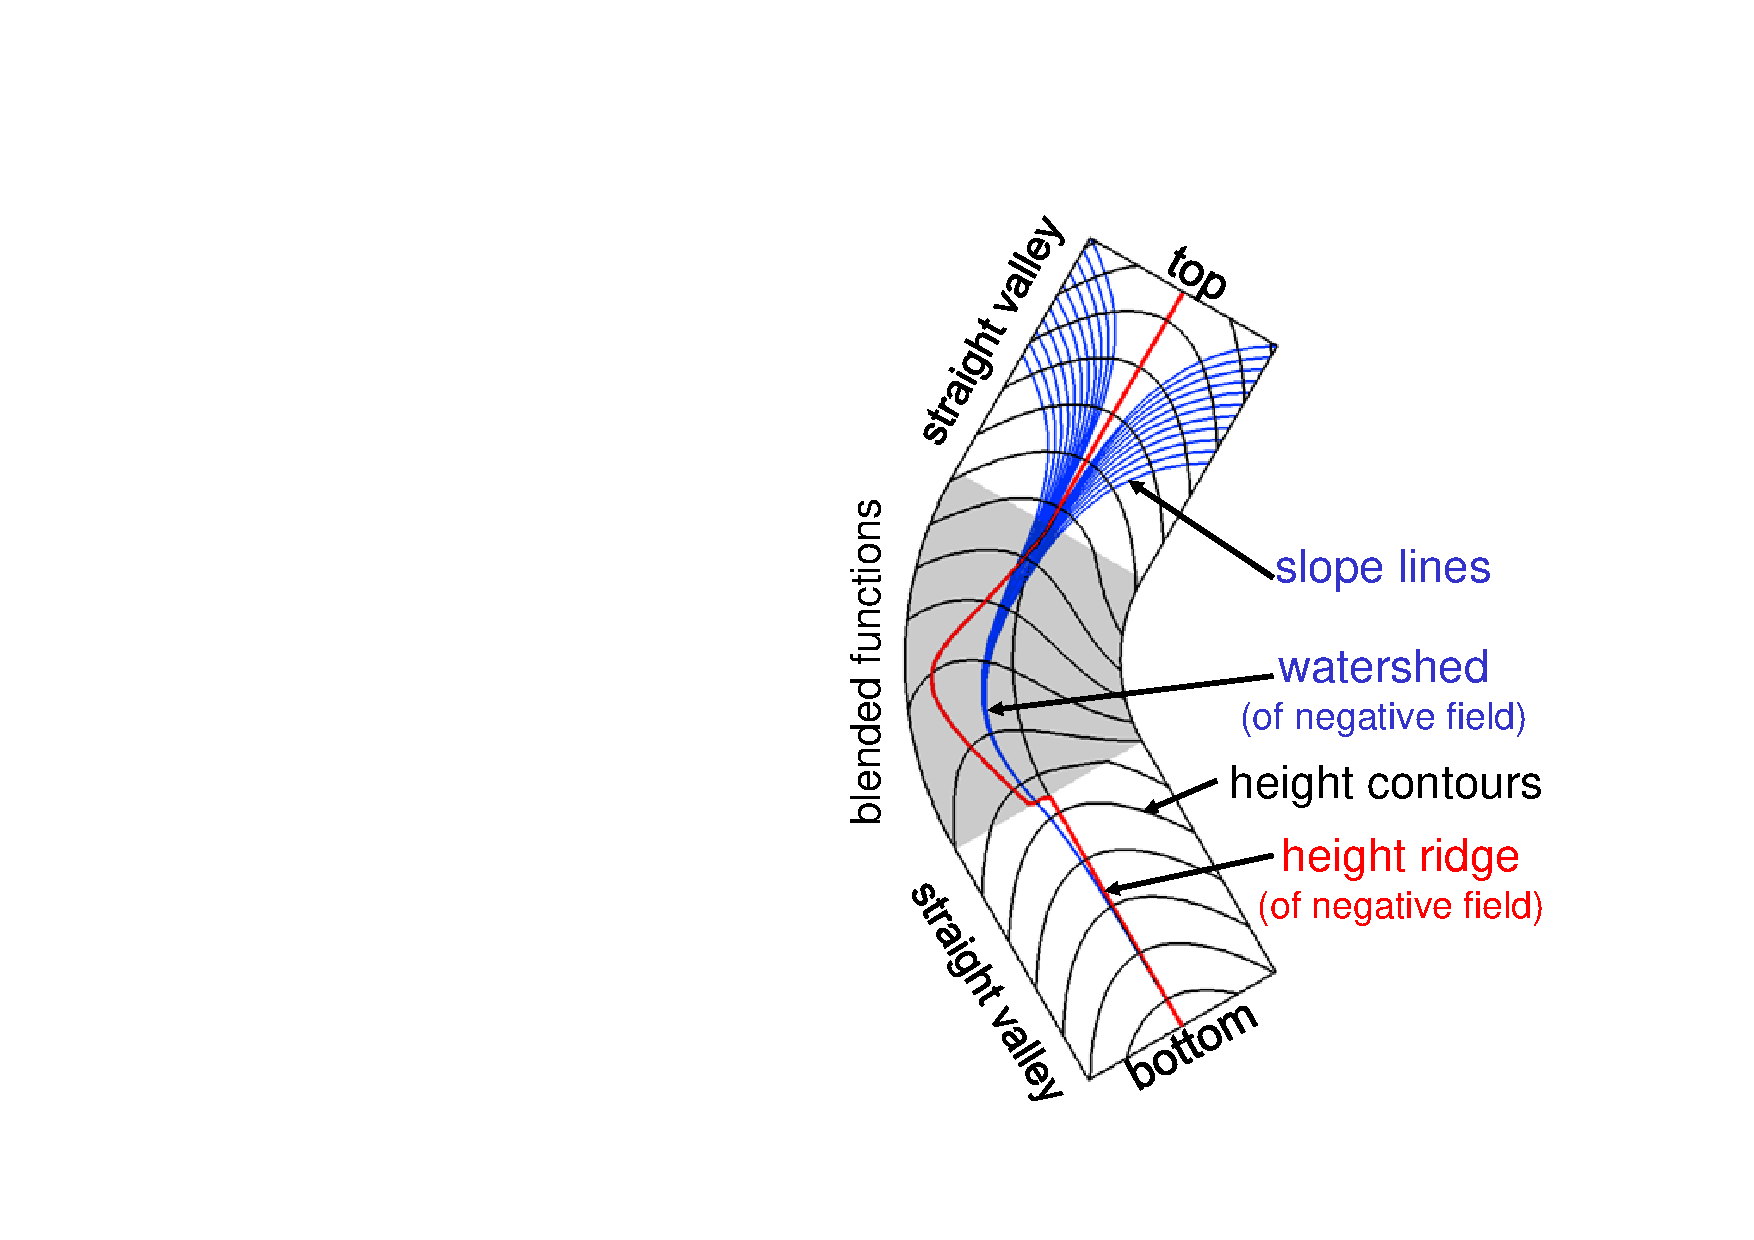
\includegraphics[width=0.4\textwidth]{img/07_blended_height_fields_example}
\end{figure}

\subsubsection{Watersheds vs. Height Ridges}
The discussion of watersheds vs. height ridges started in computer vision (Koendrick/van Doorn 1993) and is still ongoing.

Watersheds:
\begin{description}
\item[+] Are \emph{slope lines} of the height field (=streamlines of the gradient field).
\item[-] Depend on boundaries.
\item[-] Require existence of a saddle point.
\end{description}

Height ridges in 3D scalar fields can be used for defining/detecting \emph{vortex core lines}. These are
\begin{itemize}
    \item Height ridges (valley lines) of \emph{pressure} (Kida and Miura).
    \item Height ridges of \emph{vorticity magnitude} (Ahmad/Kenwright/Strawn).
\end{itemize}

\subsection{Geometric Features of Surfaces}
On \emph{surfaces} in 3-space, 0- and 1-dimensional features can by defined by the (differential) geometry alone. 


The term "ridge can refer to either height ridges or curvature ridges. Curvature ridges are not appropriate as features of a scalar field (height field).
Reasons:
\begin{enumerate}
    \item Invariance under rotation  (tilting the terrain)
    \item No invariance under scaling.
\end{enumerate}

\subsection{Line-Like Features in Vector Fields}
\paragraph{Separation lines} in boundary shear flow (Kenwright): A point $x$ lies on a \emph{separation} or \emph{raattachment line} if
\begin{enumerate}
    \item At $x$ the field vector $v(x)$ is an eigenvector of $\nabla v(x)$,
    \item the corresponding eigenvalue is the one with smaller absolute value. 
\end{enumerate}
\begin{figure}[H]
    \centering
    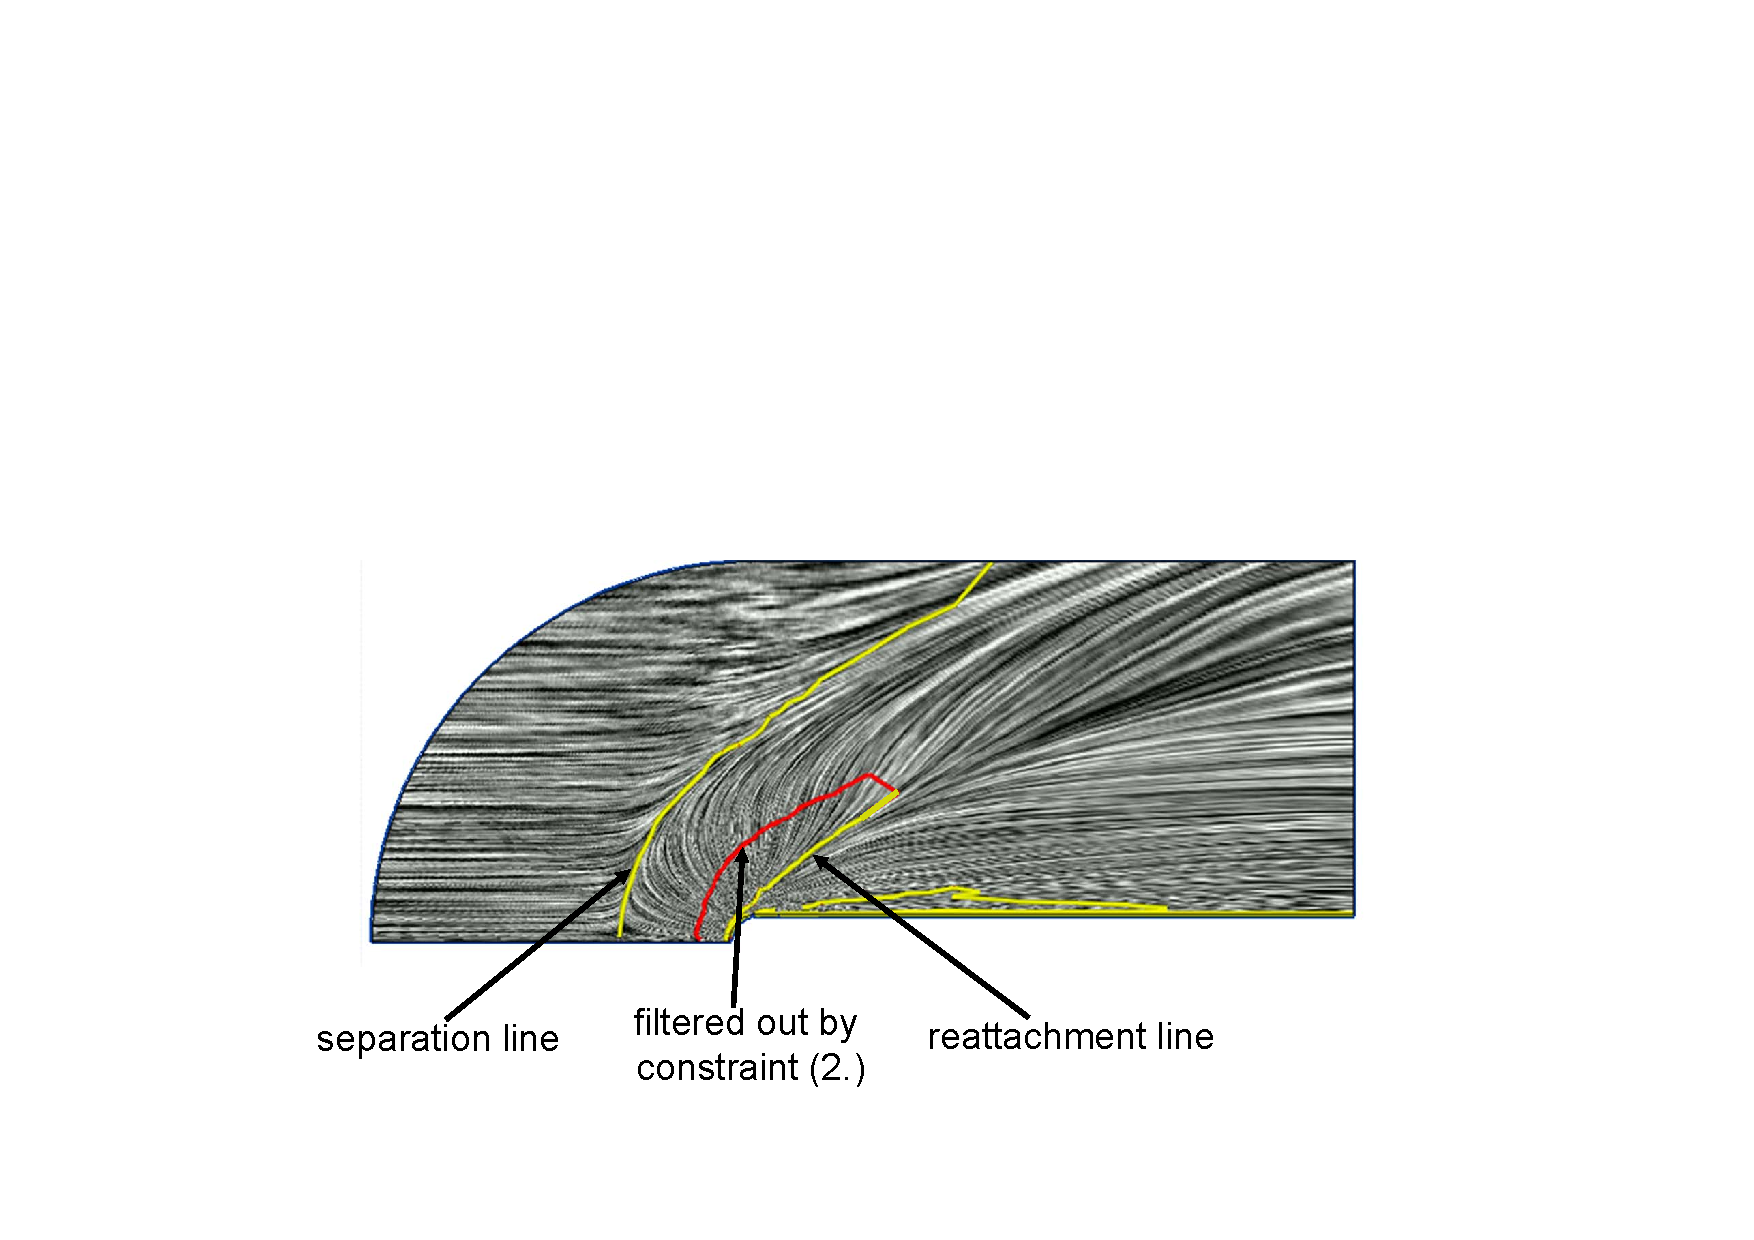
\includegraphics[width=0.7\textwidth]{img/07_separation_lines}
\end{figure}

\paragraph{Vortex core lines} (Sujudi/Haimes) A point $x$ lies on a \emph{vortex core line} if
\begin{enumerate}
    \item At $x$ the field vector $v(x)$ is an eigenvector of $\Delta v(x)$
    \item the two other eigenvalues of $\Delta v(x)$ are complex.
\end{enumerate}

Alternative definitions:
\begin{itemize}
    \item According to Levy et al., longitudinal vortices have a high normalised helicity (or small angles between velocity and vorticity).
    
        Vortex core line criterion: $v(x)$ is (anti-) parallel to $\omega (x)$.
        
    \item Singer and Banks' method:
    
        \begin{itemize}
            \item Find a first point on the core line
            \item Repeat
                \begin{itemize}
                    \item Predict the next point along $\omega (x)$
                    \item Correct to pressure minimum in normal plane of $\omega(x)$
                \end{itemize}
            \item Compute vortex hull.
        \end{itemize}
\end{itemize}

\paragraph{Computing Line-Like Featurs} Instead of computing eigenvectors for height ridges, Sujud-Haimes core lines etc. Make use of the following observation:

$v$ is an eigenvector of $A$ iff $Av$ is \emph{parallel} to $v$.

Recipe:
\begin{itemize}
    \item Compute $w = Av$ as a \emph{derived field}.
    \item Find places where $v$ and $w$ are parallel (or one of them is $0$).
    \item Apply constraints
    \item Apply post-filtering.
\end{itemize}

Parallel vectors operator: Given $v$, $w$: Returns points where $v$ and $w$ are paralllel.

Implementation:
\begin{description}
    \item 2D: $v\times w =0 $ is just a contour line problem.
    \item 3D: $v\times w=0$ is 3 equations for 3 unknowns:
        \begin{itemize}
            \item Equations are linearly dependent
            \item Can be solved with Marching Cubes like method.
        \end{itemize}
 
\end{description}

\subsection{Tracking of Features}
In time-dependent data, features are usually extracted for single time steps. Howto recognise a feature in a different time step?
Some methods are:
\begin{itemize}
    \item Decide on \emph{spatial overla} (Silver et al.)
        \begin{itemize}
            \item Appropriate for region-type features
            \item Detects motion and events (split, merge, birth, death)
        \end{itemize}
    \item Decide on \emph{feature attributes} (Reinders)
        \begin{itemize}
            \item Use attributes such as position, shape (fitted ellipsoid), orientation, spin, data values, etc...
            \item Combine with motion prediction.
        \end{itemize}
\end{itemize}

\subsection{Post-Filtering of Features}
\begin{description}
\item Specific for ridges:

    Height $>$ Threshold
\item Specific for vortex axes:

    Vortex strength $>$ Threshold
    
\item General line-type features:

    \begin{description}
        \item Angle (line, vector) $<$ Threshold
        \item Length (line) $>$ Threshold
    \end{description}
\end{description}



















